\chapter{浮动体}

\section{插图}

插图功能是利用 \TeX\ 的特定编译程序提供的机制实现的,不同的编译程序支持不同的图形方式。有的同学可能听说“\LaTeX\ 只支持 EPS”,事实上这种说法是不准确的。\XeTeX 可以很方便地插入 EPS、PDF、PNG、JPEG、JPG 格式的图片。

一般图形都是处在浮动环境中。之所以称为浮动是指最终排版效果图形的位置不一定与源文件中的位置对应,这也是刚使用 \LaTeX\ 同学可能遇到的问题。如果要强制固定浮动图形的位置,请使用 \pkg{float} 宏包,它提供了 \texttt{[H]} 参数。

\subsection{单个图形}

图要有图注,并置于图的编号之后,图的编号和图注应置于图下方的居中位置。引用图应在图题右上角标出文献来源。当插图中组成部件由数字或字母等编号表示时,可在插图下方添加图注进行说明,如图~\ref{fig:shmtu-school-motto} 所示。一般来说,研究生图注与表注一般要求中英文对照。但是由于上海海事大学没有明确要求,故推荐仅使用中文图注。若有需要添加双语图注,用法如图~\ref{fig:shmtu-school-motto-2}所示。

\begin{figure}[!htp]
	\centering
	
\includegraphics[width=10cm]{shmtu-school-motto}
	\caption{王伯群校长与吴淞商船校训}
	\label{fig:shmtu-school-motto}
\end{figure}

\begin{figure}[!htp]
	\centering
	
\includegraphics[width=10cm]{shmtu-school-motto}
	\bicaption{王伯群校长与吴淞商船校训}{President Wang Boqun and the school motto of WuSong Merchant Shipping}
	\label{fig:shmtu-school-motto-2}
\end{figure}

\subsection{多个图形}

简单插入多个图形的例子如图~\ref{fig:parallel-1} 所示。这两个水平并列放置的子图共用一个图形计数器,没有各自的子图题。

\begin{figure}[!htp]
  \centering
  
\includegraphics[height=2cm]{images/shmtu-badge}
  \hspace{1cm}
  
\includegraphics[height=2cm]{images/shmtu-badge}
  \caption{上海海事大学校徽}
  \label{fig:parallel-1}
\end{figure}

如果多个图形相互独立,并不共用一个图形计数器,那么用 \cs{minipage} 或者\cs{parbox} 就可以,如图~\ref{fig:parallel-2-1} 与图~\ref{fig:parallel-2-2}。

\begin{figure}[!htp]
  \begin{minipage}{0.48\textwidth}
  	\centering
    
\includegraphics[height=1.5cm]{images/shmtu-badge.jpg}
    \caption{并排第一个图}
    \label{fig:parallel-2-1}
  \end{minipage}
  \hfill
  \begin{minipage}{0.48\textwidth}
    \centering
    
\includegraphics[height=1.5cm]{images/shmtu-badge.jpg}
    \caption{并排第二个图}
    \label{fig:parallel-2-2}
  \end{minipage}
\end{figure}

如果要为共用一个计数器的多个子图添加子图注,那么使用\cs{subcaptionbox}(双语图注使用\cs{bisubcaptionbox})并排子图,子图注置于子图之下,子图号用 (a)、(b)、(c)等表示。如图~\ref{fig:subcaptionbox}、图~\ref{fig:subcaptionbox-a}、图~\ref{fig:subcaptionbox-b}、图~\ref{fig:subcaptionbox-c}所示。

\begin{figure}[!htp]
  \subcaptionbox{上海海事大学校徽\label{fig:subcaptionbox-a}}%
	[0.5\textwidth]{%
	  
\includegraphics[height=1.5cm]{images/shmtu-badge}
	}
  \hfill
  \subcaptionbox{上海海事大学校名\label{fig:subcaptionbox-b}}%
    [0.5\textwidth]{%
	  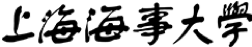
\includegraphics[width=0.5\textwidth]{images/shmtu-name}
	}
  \hfill
  \subcaptionbox{上海海事大学校徽\label{fig:subcaptionbox-c}}%
    [\textwidth]{%
	  
\includegraphics[height=1.5cm]{images/shmtu-badge}
  }
  \caption{共用一个计数器的多个子图图注}
  \label{fig:subcaptionbox}
\end{figure}

\section{表格}

\subsection{基本表格}

编排表格应简单明了,表达一致,明晰易懂,表文呼应、内容一致。表注置于表上,研究生学位论文可以用中、英文两种文字居中排写,中文在上,也可以只用中文。

表格的编排采用国际通行的三线表\footnote{三线表,以其形式简洁、功能分明、阅读方便而在科技论文中被推荐使用。三线表通常只有 3 条线,即顶线、底线和栏目线,没有竖线。}。三线表可以使用 \pkg{booktabs} 提供的 \cs{toprule}、\cs{midrule} 和 \cs{bottomrule}。它们与 \pkg{longtable} 能很好的配合使用。

\begin{table}[!htp]
  \centering
  \caption[一个标准的三线表]{一个标准的三线表\footnotemark}
  \label{tab:firstone}
  \begin{tabular}{llr}  
    \toprule
    \multicolumn{2}{c}{Item} \\
    \cmidrule(r){1-2}
    Animal    & Description & Price (\$) \\
    \midrule
    Gnat      & per gram    & 13.65      \\
              &    each     & 0.01       \\
    Gnu       & stuffed     & 92.50      \\
    Emu       & stuffed     & 33.33      \\
    Armadillo & frozen      & 8.99       \\
    \bottomrule
  \end{tabular}
\end{table}
\footnotetext{这个例子来自
  \href{https://mirrors.sjtug.sjtu.edu.cn/ctan/macros/latex/contrib/booktabs/booktabs.pdf}%
  {《Publication quality tables in LaTeX》}(\pkg{booktabs} 宏包的文档)。这也是
  一个在表格中使用脚注的例子,请留意与 \pkg{threeparttable} 实现的效果有何不
  同。}
  
\subsection{复杂表格}

我们经常会在表格下方标注数据来源,或者对表格里面的条目进行解释。可以用\pkg{threeparttable} 实现带有脚注的表格,如表~\ref{tab:footnote}。

\begin{table}[!htpb]
  \bicaption{一个带有脚注的表格的例子}{A Table with footnotes}
  \label{tab:footnote}
  \centering
  \begin{threeparttable}[b]
     \begin{tabular}{ccd{4}cccc}
      \toprule
      \multirow{2}*{total} & \multicolumn{2}{c}{20\tnote{a}} & \multicolumn{2}{c}{40} & \multicolumn{2}{c}{60} \\
      \cmidrule(lr){2-3}\cmidrule(lr){4-5}\cmidrule(lr){6-7}
      & www & \multicolumn{1}{c}{k} & www & k & www & k \\ % 使用说明符 d 的列会自动进入数学模式,使用 \multicolumn 对文字表头做特殊处理
      \midrule
      & $\underset{(2.12)}{4.22}$ & 120.0140\tnote{b} & 333.15 & 0.0411 & 444.99 & 0.1387 \\
      & 168.6123 & 10.86 & 255.37 & 0.0353 & 376.14 & 0.1058 \\
      & 6.761    & 0.007 & 235.37 & 0.0267 & 348.66 & 0.1010 \\
      \bottomrule
    \end{tabular}
    \begin{tablenotes}
      \item [a] the first note.% or \item [a]
      \item [b] the second note.% or \item [b]
    \end{tablenotes}
  \end{threeparttable}
\end{table}

\zhlipsum[1]

如某个表需要转页接排,可以用 \pkg{longtable} 实现。接排时表注省略,表头应重复书写,并在右上方写“续表 xx”,如表~\ref{tab:grid_mlmmh}。

\begin{longtable}[c]{c*{3}{r}}
  \caption[高变网格的可行三元组]{高变网格的可行三元组, MLMMH.}
  \label{tab:grid_mlmmh} \\
  % 表头
  \toprule
  \multicolumn{1}{c}{Time (s)} & \multicolumn{1}{c}{Triple chosen} & \multicolumn{1}{c}{Other feasible triples} \\
  \midrule
  \endfirsthead
	
  % 续表
  \multicolumn{3}{r}{续表~\thetable} \\
  \toprule
  % 续表表头
  \multicolumn{1}{c}{\textbf{Time (s)}} & \multicolumn{1}{c}{\textbf{Triple chosen}} & \multicolumn{1}{c}{\textbf{Other feasible triples}} \\ 
  \midrule
  \endhead

  \midrule
  \multicolumn{3}{r}{续下页} \\
  \endfoot
  
  \bottomrule
  \endlastfoot
  
0 & (1, 11, 13725) & (1, 12, 10980), (1, 13, 8235), (2, 2, 0), (3, 1, 0) \\
2745 & (1, 12, 10980) & (1, 13, 8235), (2, 2, 0), (2, 3, 0), (3, 1, 0) \\
5490 & (1, 12, 13725) & (2, 2, 2745), (2, 3, 0), (3, 1, 0) \\
8235 & (1, 12, 16470) & (1, 13, 13725), (2, 2, 2745), (2, 3, 0), (3, 1, 0) \\
10980 & (1, 12, 16470) & (1, 13, 13725), (2, 2, 2745), (2, 3, 0), (3, 1, 0) \\
13725 & (1, 12, 16470) & (1, 13, 13725), (2, 2, 2745), (2, 3, 0), (3, 1, 0) \\
16470 & (1, 13, 16470) & (2, 2, 2745), (2, 3, 0), (3, 1, 0) \\
19215 & (1, 12, 16470) & (1, 13, 13725), (2, 2, 2745), (2, 3, 0), (3, 1, 0) \\
21960 & (1, 12, 16470) & (1, 13, 13725), (2, 2, 2745), (2, 3, 0), (3, 1, 0) \\
24705 & (1, 12, 16470) & (1, 13, 13725), (2, 2, 2745), (2, 3, 0), (3, 1, 0) \\
27450 & (1, 12, 16470) & (1, 13, 13725), (2, 2, 2745), (2, 3, 0), (3, 1, 0) \\
30195 & (2, 2, 2745) & (2, 3, 0), (3, 1, 0) \\
32940 & (1, 13, 16470) & (2, 2, 2745), (2, 3, 0), (3, 1, 0) \\
35685 & (1, 13, 13725) & (2, 2, 2745), (2, 3, 0), (3, 1, 0) \\
38430 & (1, 13, 10980) & (2, 2, 2745), (2, 3, 0), (3, 1, 0) \\
41175 & (1, 12, 13725) & (1, 13, 10980), (2, 2, 2745), (2, 3, 0), (3, 1, 0) \\
43920 & (1, 13, 10980) & (2, 2, 2745), (2, 3, 0), (3, 1, 0) \\
46665 & (2, 2, 2745) & (2, 3, 0), (3, 1, 0) \\
49410 & (2, 2, 2745) & (2, 3, 0), (3, 1, 0) \\
52155 & (1, 12, 16470) & (1, 13, 13725), (2, 2, 2745), (2, 3, 0), (3, 1, 0) \\
54900 & (1, 13, 13725) & (2, 2, 2745), (2, 3, 0), (3, 1, 0) \\
57645 & (1, 13, 13725) & (2, 2, 2745), (2, 3, 0), (3, 1, 0) \\
60390 & (1, 12, 13725) & (2, 2, 2745), (2, 3, 0), (3, 1, 0) \\
63135 & (1, 13, 16470) & (2, 2, 2745), (2, 3, 0), (3, 1, 0) \\
65880 & (1, 13, 16470) & (2, 2, 2745), (2, 3, 0), (3, 1, 0) \\
68625 & (2, 2, 2745) & (2, 3, 0), (3, 1, 0) \\
71370 & (1, 13, 13725) & (2, 2, 2745), (2, 3, 0), (3, 1, 0) \\
74115 & (1, 12, 13725) & (2, 2, 2745), (2, 3, 0), (3, 1, 0) \\
76860 & (1, 13, 13725) & (2, 2, 2745), (2, 3, 0), (3, 1, 0) \\
79605 & (1, 13, 13725) & (2, 2, 2745), (2, 3, 0), (3, 1, 0) \\
82350 & (1, 12, 13725) & (2, 2, 2745), (2, 3, 0), (3, 1, 0) \\
85095 & (1, 12, 13725) & (1, 13, 10980), (2, 2, 2745), (2, 3, 0), (3, 1, 0) \\
87840 & (1, 13, 16470) & (2, 2, 2745), (2, 3, 0), (3, 1, 0) \\
\end{longtable}


\section{算法环境}

算法环境可以使用 \pkg{algorithms} 宏包或者较新的 \pkg{algorithm2e} 实现。算法~\ref{algo:algorithm} 是一个使用 \pkg{algorithm2e} 的例子。关于排版算法环境的具体方法,请阅读相关宏包的官方文档\footnote{\url{http://tug.ctan.org/macros/latex/contrib/algorithm2e/doc/algorithm2e.pdf}}。

\begin{algorithm}
  \DontPrintSemicolon % Some LaTeX compilers require you to use \dontprintsemicolon instead
  \KwIn{A finite set $A=\{a_1, a_2, \ldots, a_n\}$ of integers}
  \KwOut{The largest element in the set}
  
  $max \gets a_1$\;
  \For{$i \gets 2$ \textbf{to} $n$} {
    \eIf{$a_i > max$} {
      $max \gets a_i$\;
    }{
      pass\;
    }
  }
  \Return{$max$}\;
  \caption{{\sc Max} finds the maximum number}
  \label{algo:algorithm}
\end{algorithm}

\section{代码环境}

我们可以在论文中插入算法,但是不建议插入大段的代码。如果确实需要插入代码,建议使用 \pkg{listings} 宏包。

\begin{codeblock}[language=Python]
# -*- coding: utf-8 -*-
import click

from app.extensions import db
from app.models import Role


def register_commands(app):
    @app.cli.command()
    @click.option('--drop', is_flag=True, help='删除之前的表后再初始化.')
    def initdb(drop):
        """初始化数据库."""
        if drop:
            click.confirm('执行该命令将会删除当前数据库,确定要执行吗?', abort=True)
            db.drop_all()
            click.echo('删除所有表.')
        db.create_all()
        click.echo('初始化数据库.')

    @app.cli.command()
    def init():
        """初始化项目"""
        click.echo('初始化数据库...')
        db.create_all()
        
        click.echo('初始化用户角色与权限...')
        Role.init_role()

        click.echo('初始化完毕.')
\end{codeblock}

